\chapter{Results}\label{cha:results}
\section{Threshold Scan Results}
For the threshold scan, the threshold was scanned in steps of 1 for a range of high gains,
starting with gain 58 and ending with the maxmial gain of 62.
\newline
The number of hits was measured for each of the 32 channels of the Citiroc1A ASICs with an integration time of \SI{400}{\milli\second}.
The threshold scan was performed for both the Citiroc1A ASICs of FPGA 1 and 2.
\newline
The results of the threshold scan are shown for the Citiroc1A ASICs of FPGA 1 and 2 for gains 58 to 62 in Figures \ref{fig:threshold_scan_58}, \ref{fig:threshold_scan_59}, \ref{fig:threshold_scan_60}, \ref{fig:threshold_scan_61} and \ref{fig:threshold_scan_62} respectively.

    \begin{figure}
        \centering
        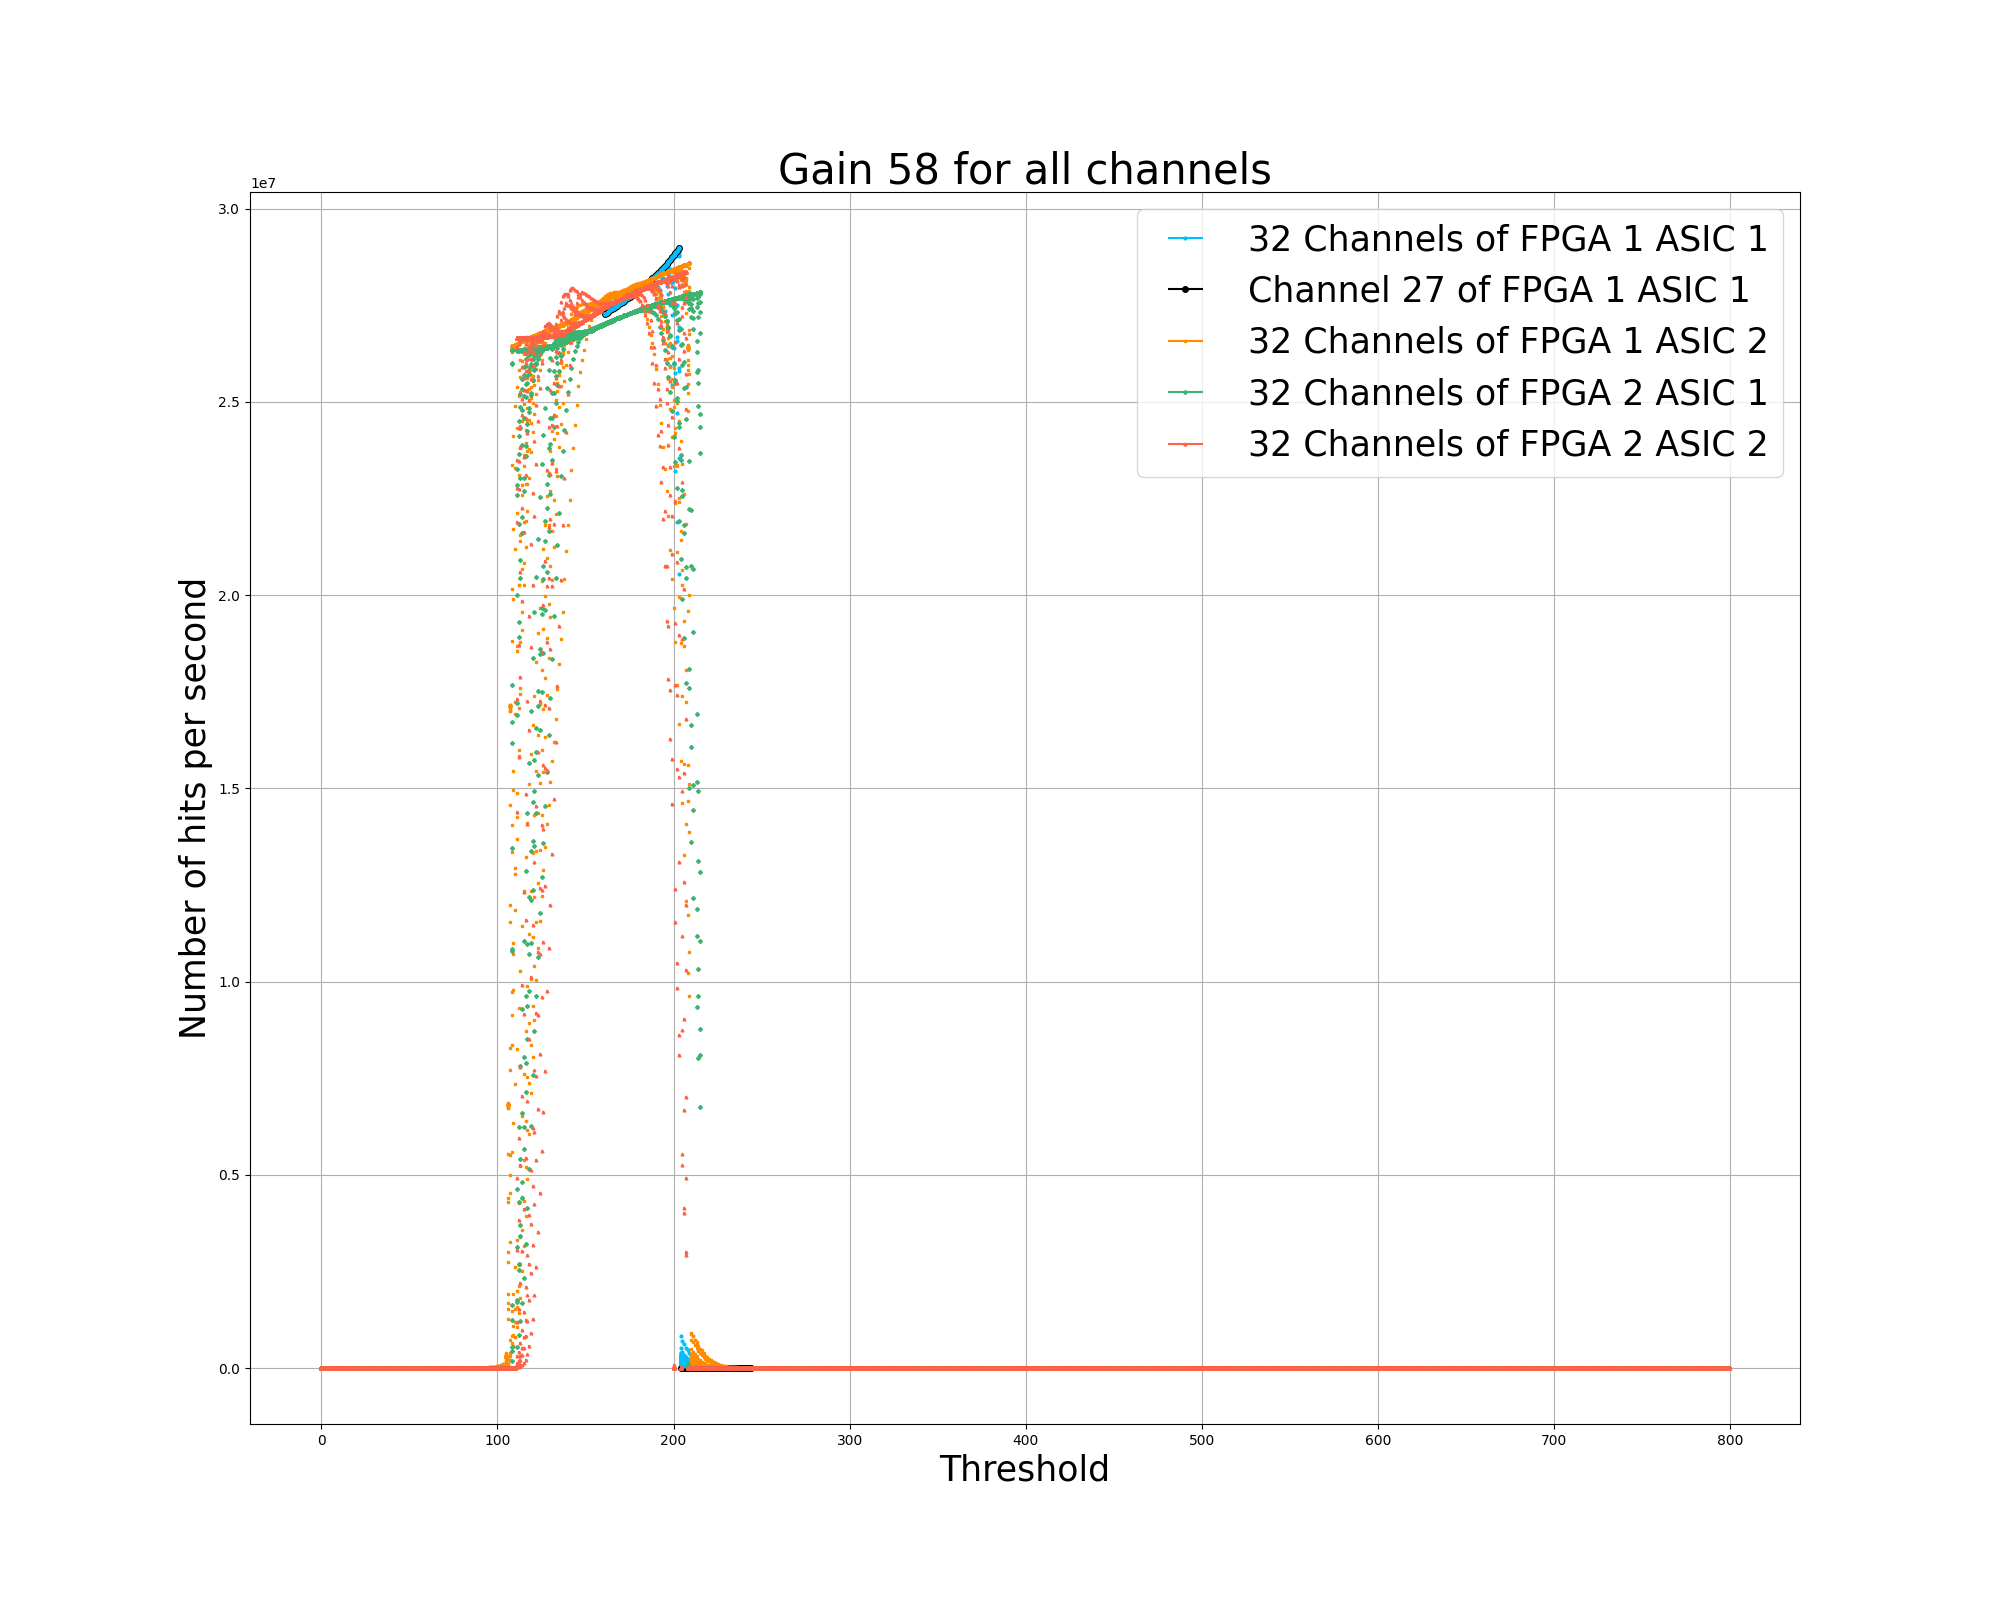
\includegraphics[width=1.0\textwidth]{Gain_58.0_ALLCHANNELS.png}
        \caption{Threshold scan of the Citiroc1A ASICs of FPGA 1 and 2 for gain 58 from threshold 0 to 800.}
        \label{fig:threshold_scan_58}
    \end{figure}
    
    \begin{figure}
        \centering
        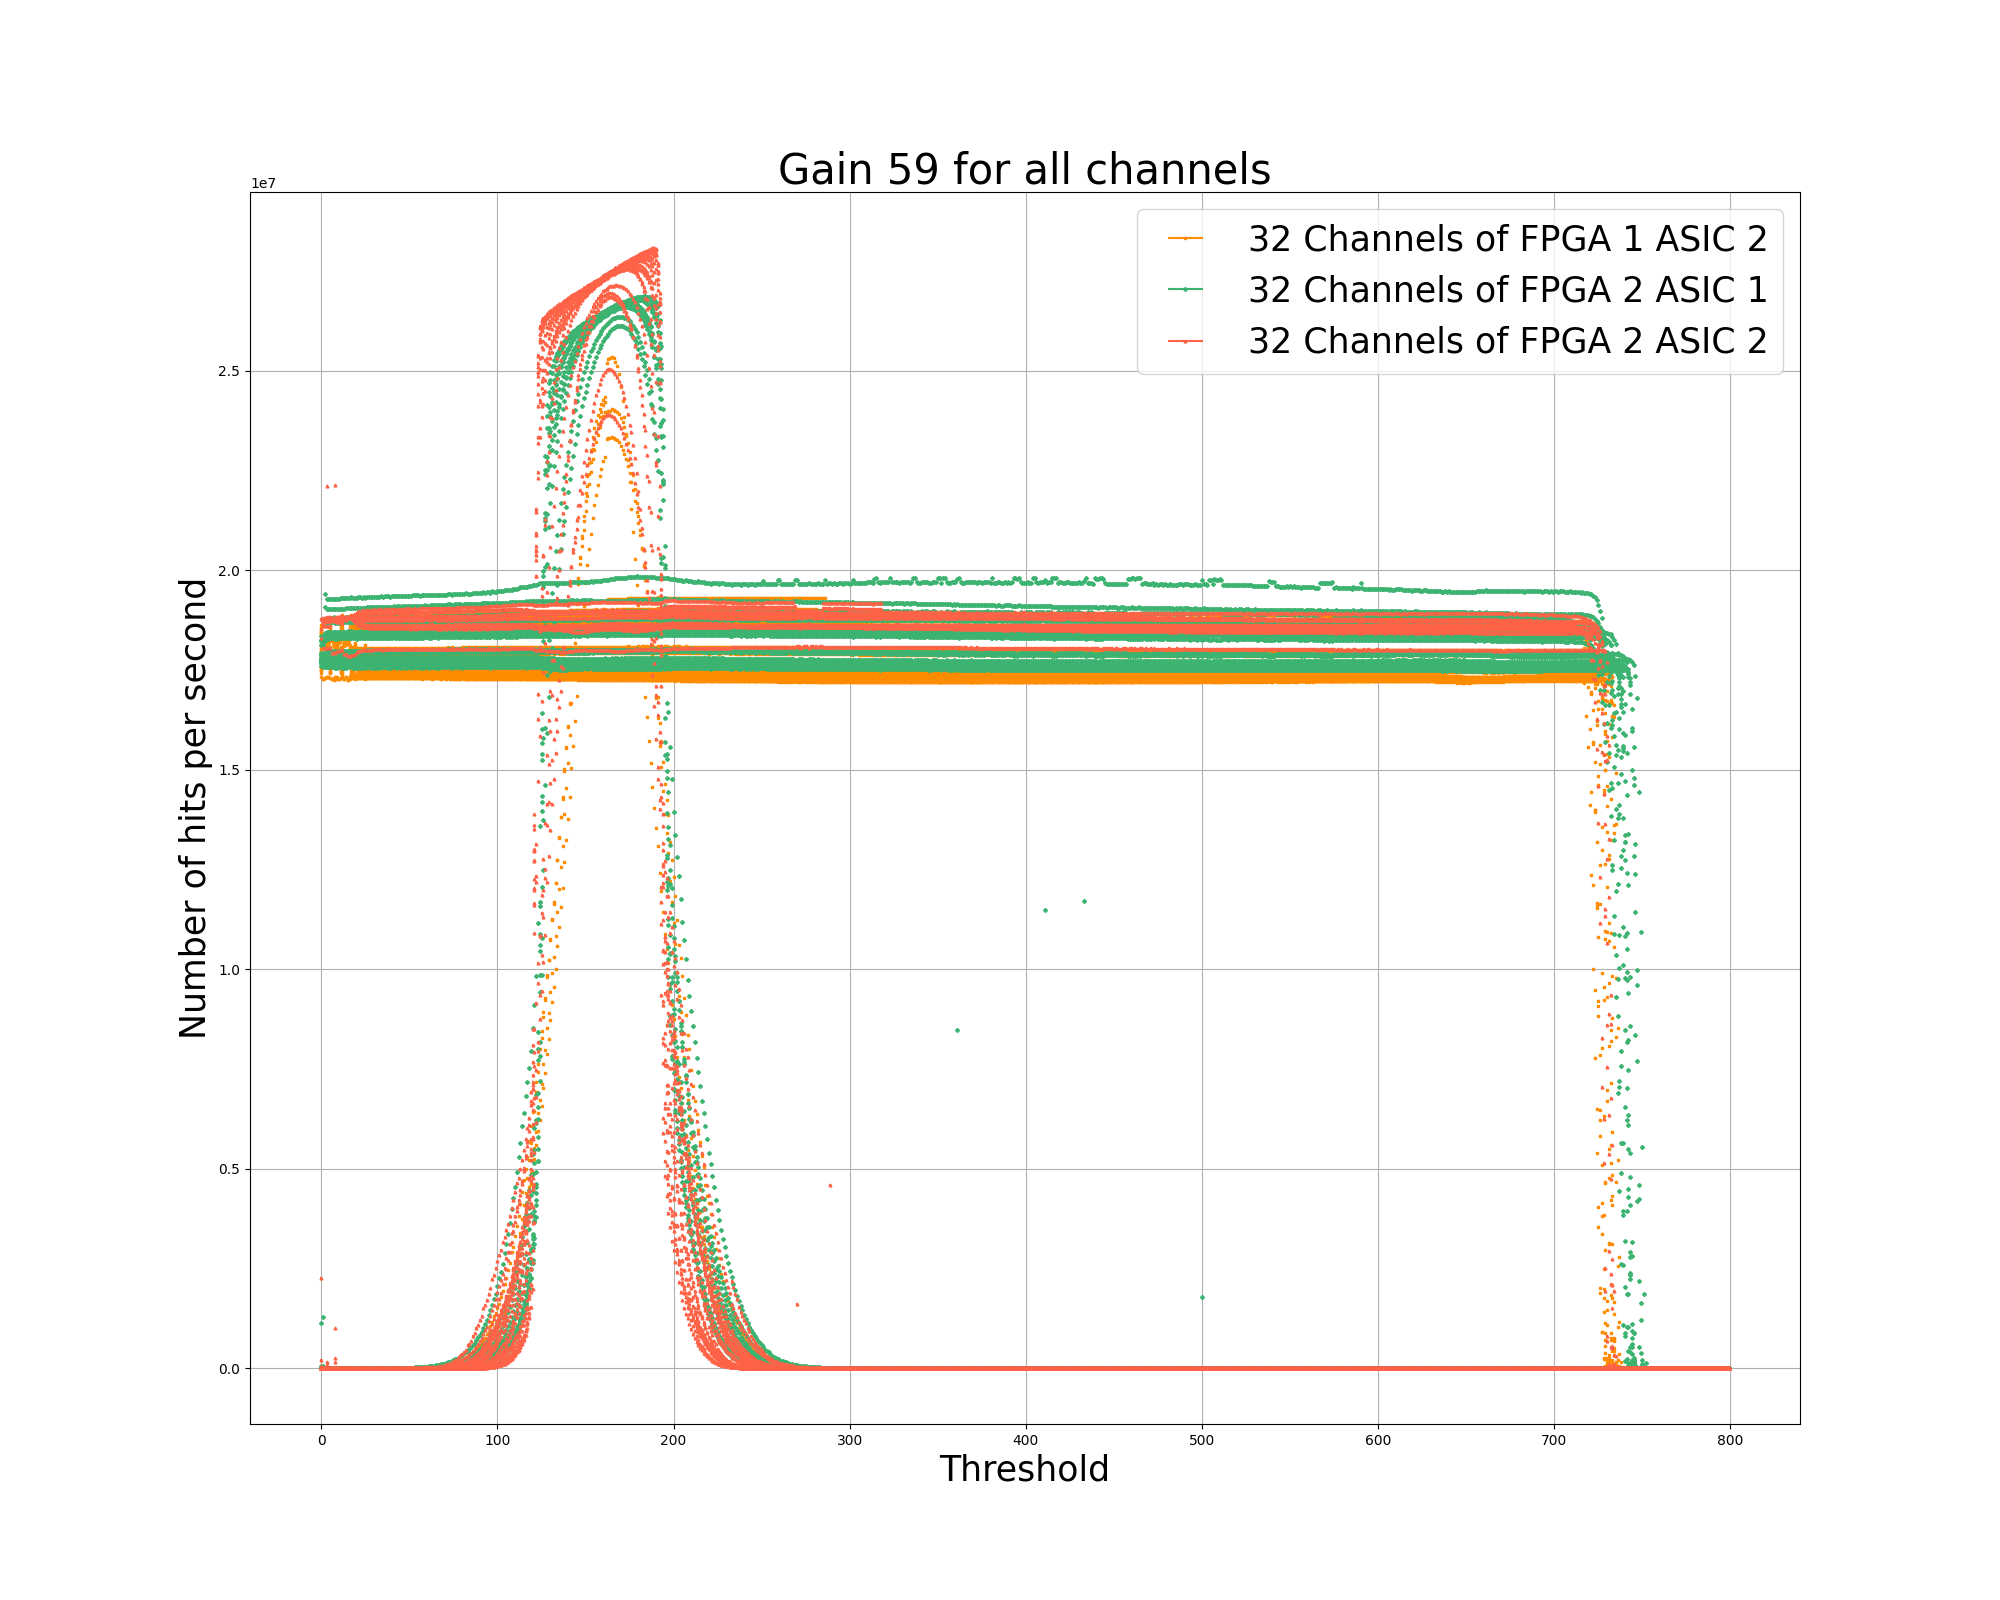
\includegraphics[width=1.0\textwidth]{Gain_59.0_ALLCHANNELS.png}
        \caption{Threshold scan of the Citiroc1A ASICs of FPGA 1 and 2 for gain 59 from threshold 0 to 800.}
        \label{fig:threshold_scan_59}
    \end{figure}
    
    \begin{figure}
        \centering
        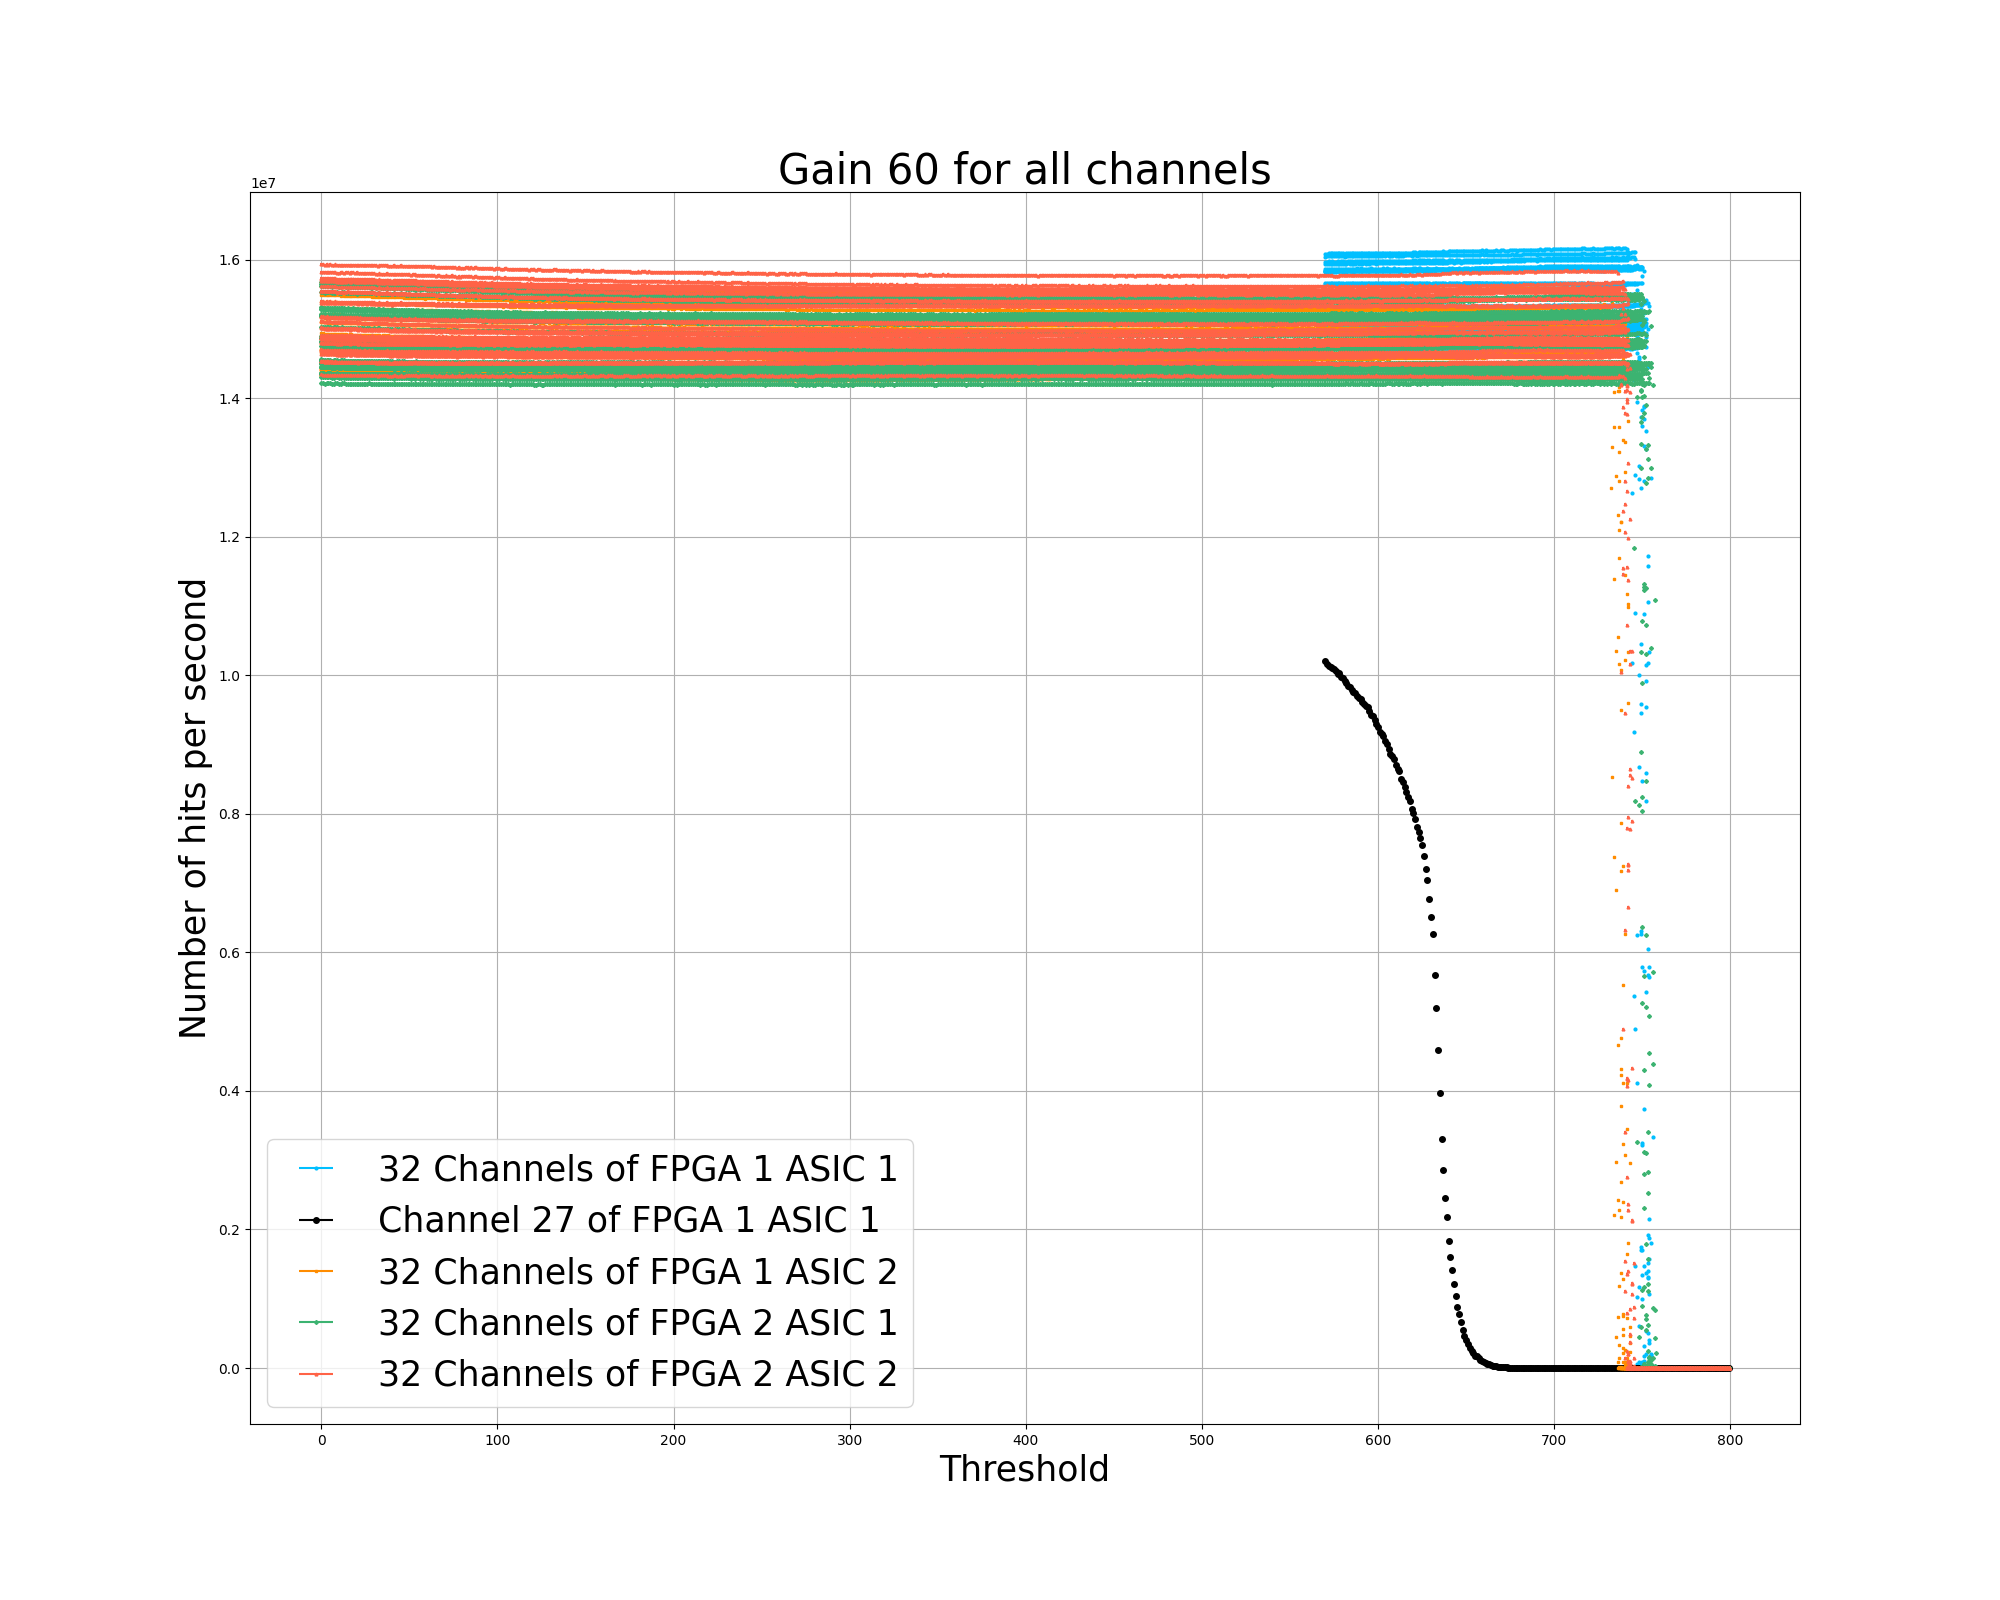
\includegraphics[width=1.0\textwidth]{Gain_60.0_ALLCHANNELS.png}
        \caption{Threshold scan of the Citiroc1A ASICs of FPGA 1 and 2 for gain 60 from threshold 0 to 800.}
        \label{fig:threshold_scan_60}
    \end{figure}
    
    \begin{figure}
        \centering
        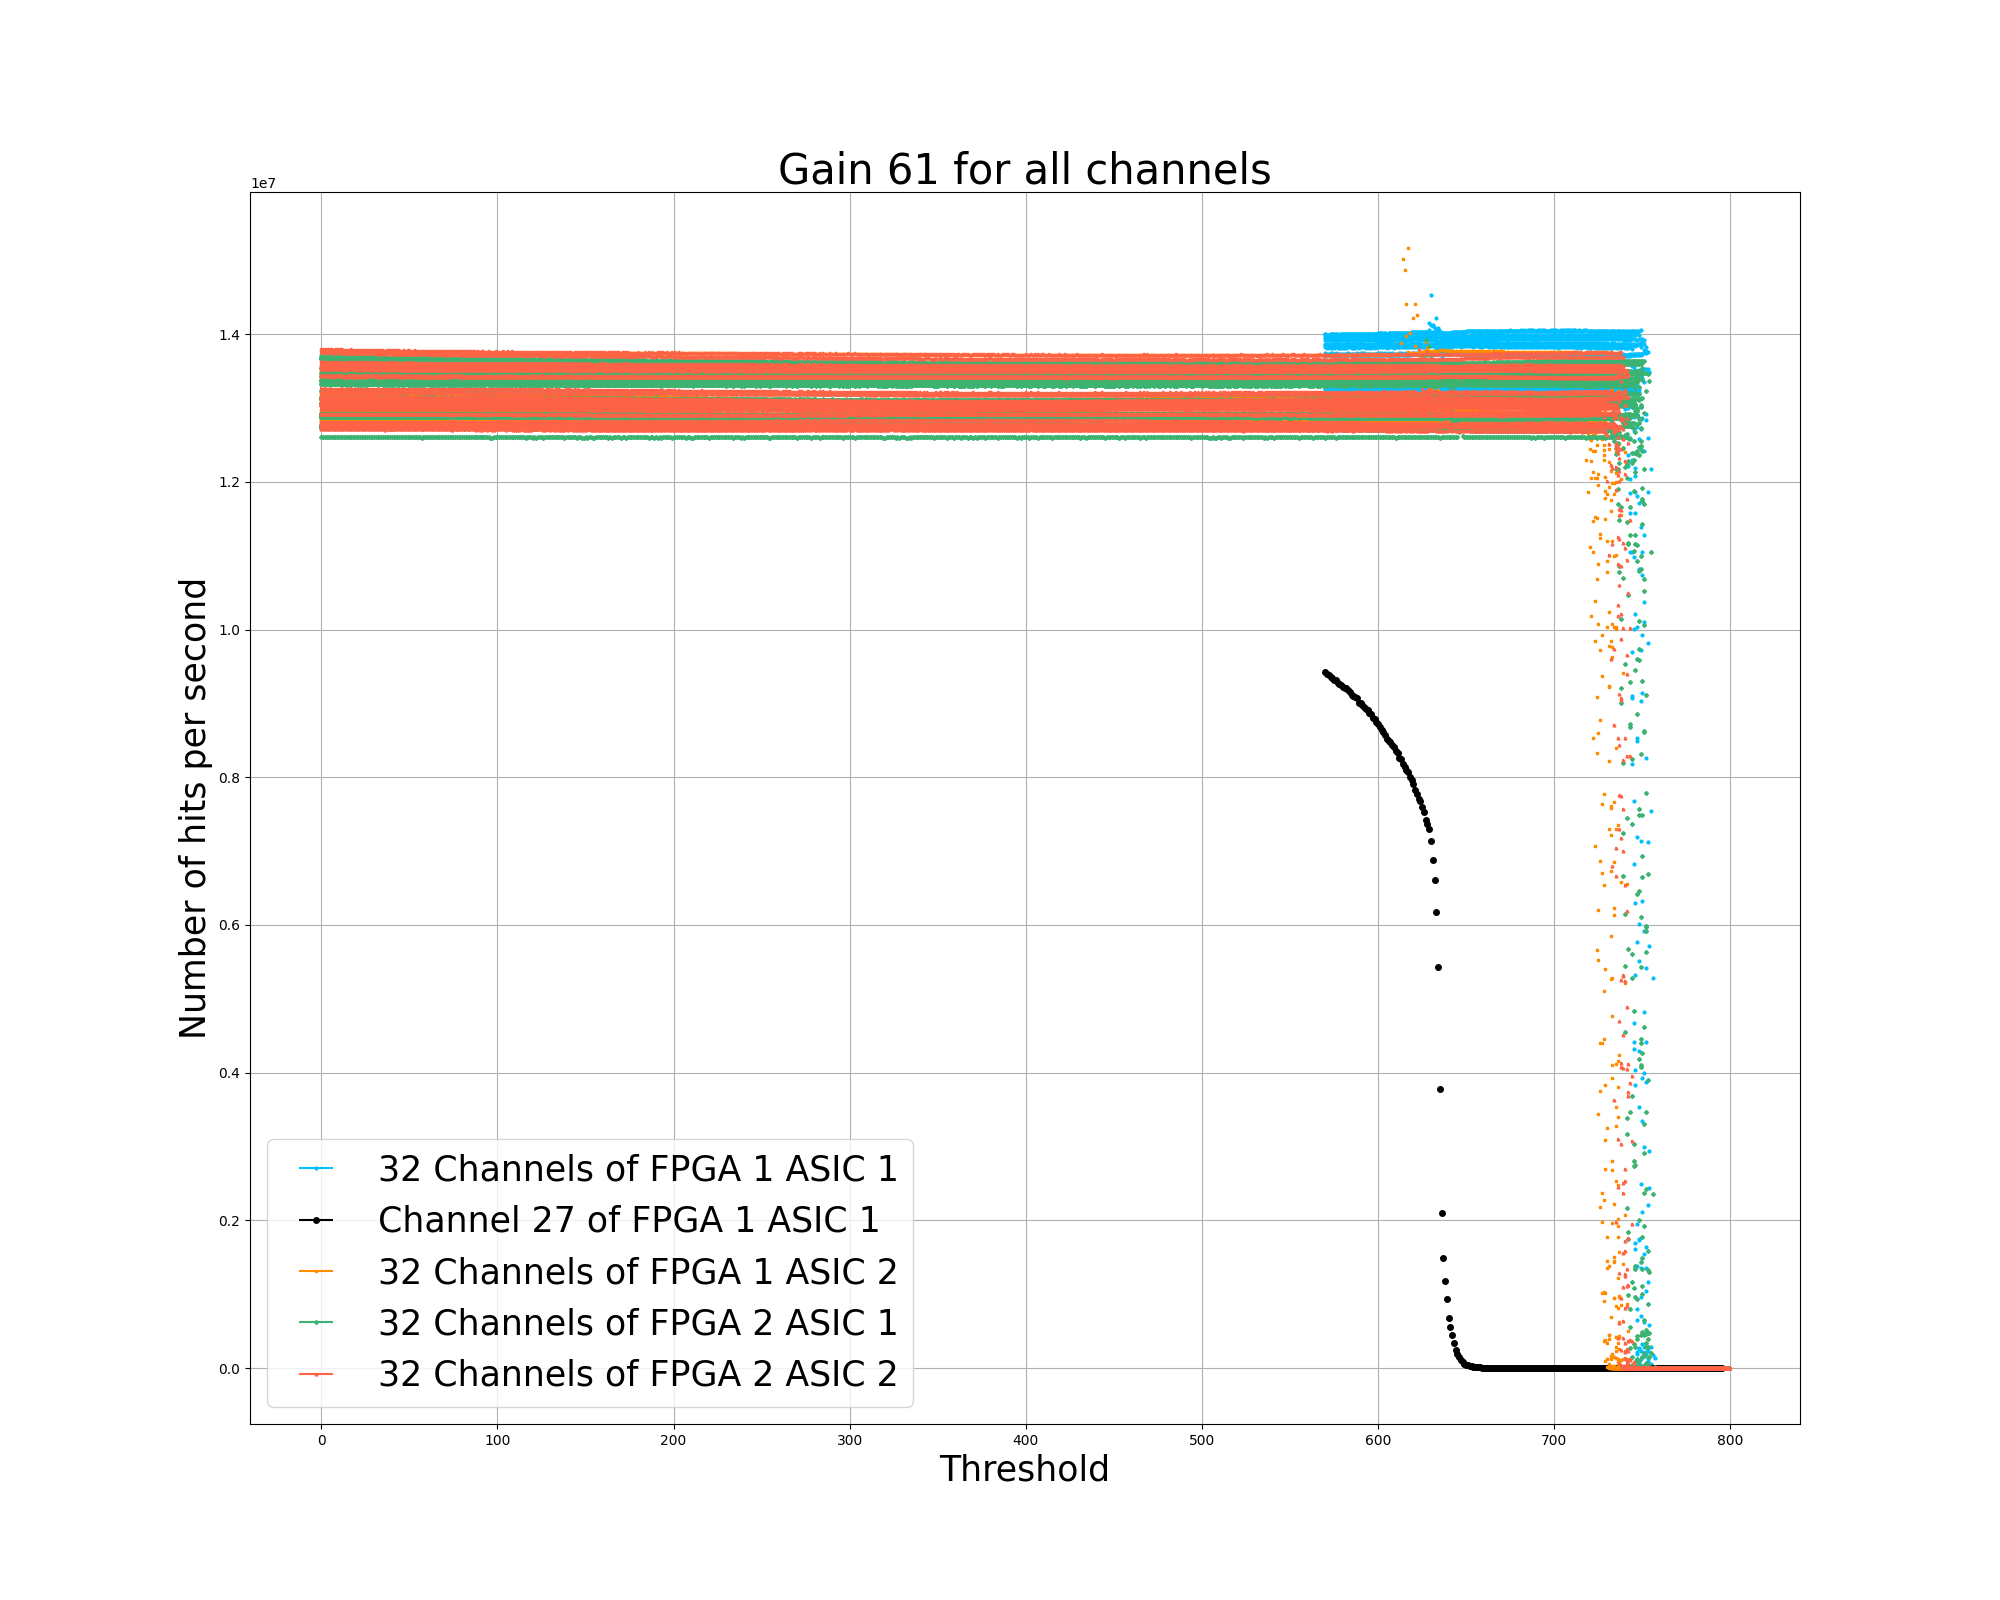
\includegraphics[width=1.0\textwidth]{Gain_61.0_ALLCHANNELS.png}
        \caption{Threshold scan of the Citiroc1A ASICs of FPGA 1 and 2 for gain 61 from threshold 0 to 800.}
        \label{fig:threshold_scan_61}
    \end{figure}
    
    \begin{figure}
        \centering
        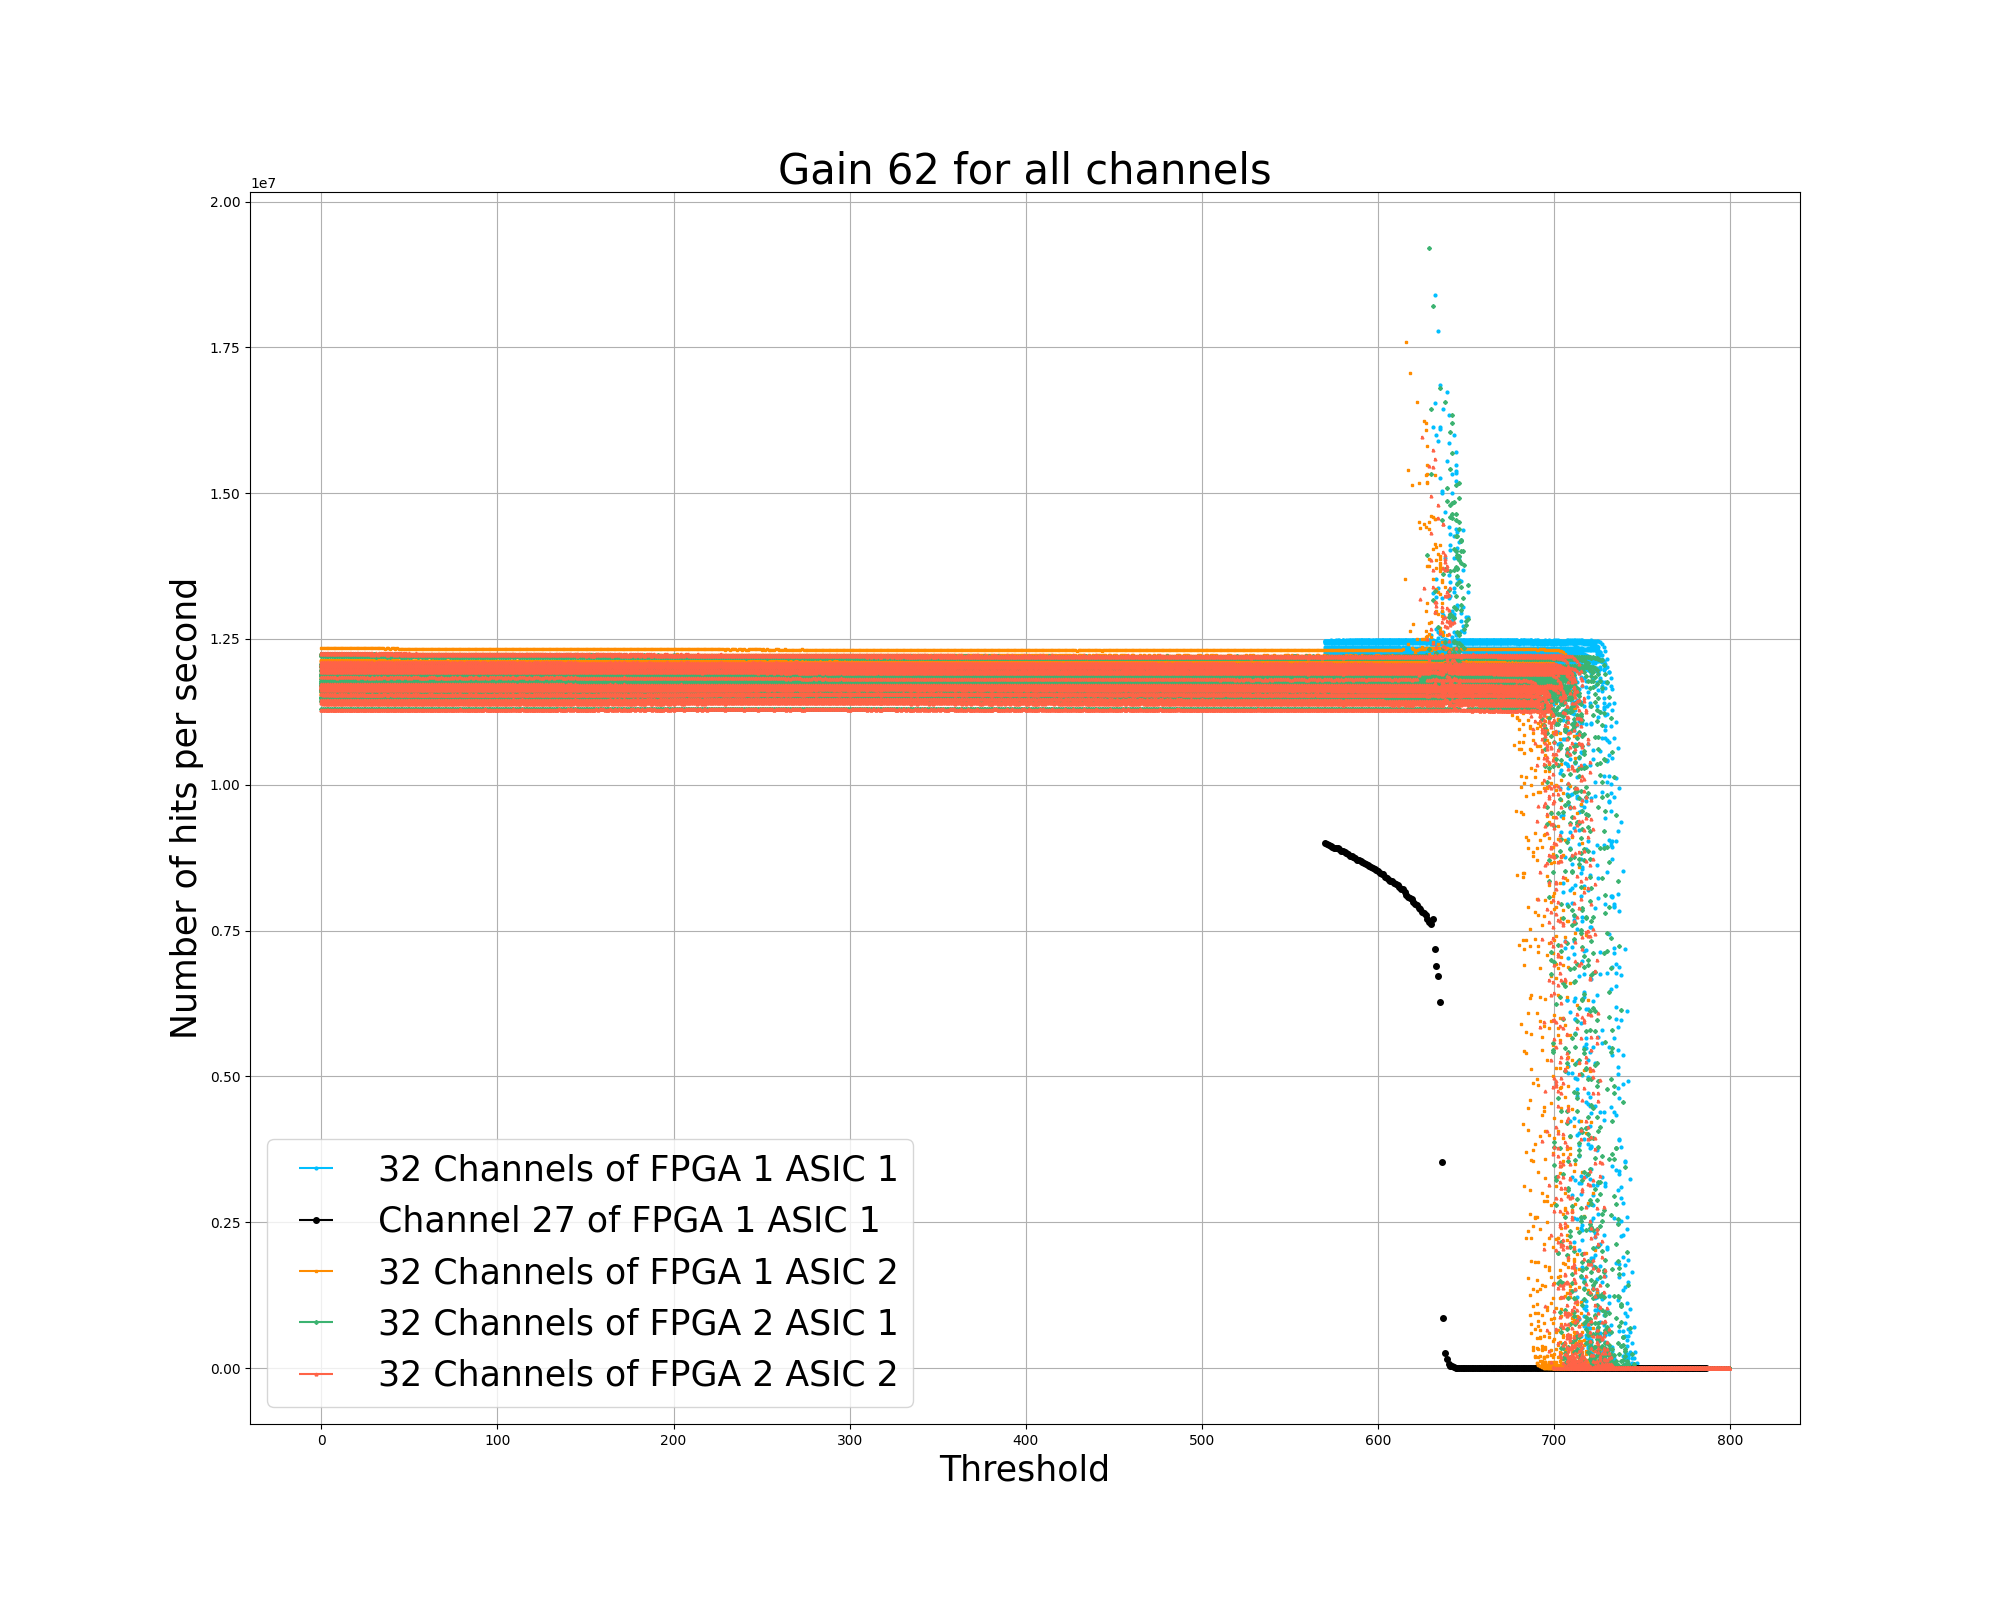
\includegraphics[width=1.0\textwidth]{Gain_62.0_ALLCHANNELS.png}
        \caption{Threshold scan of the Citiroc1A ASICs of FPGA 1 and 2 for gain 62 from threshold 0 to 800.}
        \label{fig:threshold_scan_62}
    \end{figure}
    

     
